\section{Model}
% Hvordan har vi valgt at prøve at løse problemet.
% Vi har delt problemet op i subproblemer ligesom tmseg
% Vi har prøvet at bruge andre machine learning metoder
% Største forskel er at vi har givet model "rå" data i stedet for feature extraction
% Fordelen er at man ikke behøver at på forhånd finde ud af hvilke features er vigtig

% Hvilke muligheder er der for at implementere modelen. forskellige ml libraries
% Vi har valgt tensorflow

% Noget om hvorfor lstm
	% Der er flere beregninger når man bruger lstms (con)
	% Long short-term memory: Hvorfor har vi brug for LONG memory?
% Hvad gør vores model forskelligt fra tmseg

% Hvad forventer vi vores model kan gøre bedre end de modeller der allerede eksisterer?

% tegning af model!!

%  Problem delt op i 4 steps som i tmseg
% Kun 3 af stepsne er machine learning
	% Første step assigner en sandsynlighed for hver klasse til hver position i sekvens
		% Vi har gjort det med en lstm, fodret med den rå sekvens
		% Første lag embeder sekvens data i et vector rum
		% Andet lag er en bidirectionel lstm 
		% Trejde og sidste lag er et softmax layer som giver en sansynligheds fordeling af de forskellige klasser
		
	% Andet step er at give hver position en klasse ud fra dens sandsynlighed 
		% med forbehold for at helixer ikke må være for korte
		% Måske tilføje et bias til nogle af klasserne
		% Ikke machine learning men mere post processing af af første step
		
	% Trejde step er justering af enderne af helixerne
	
	% Fjerne step er finde en topologi af sekvens, 
		% ie hvilken vej vender helixerne og hvilke dele er inden for membranen og hvilke er uden for

In many \gls{ann} based models it is very hard to ensure some syntax rules for the output. If the output 
classes was \emph{\gls{tmh}}, \emph{inside} and \emph{outside}, then it should not be possible for a output sequence to contain 
adjacent positions with one being inside and the other being outside or both ends of a \gls{tmh} to be on the 
same side, but these rules cannot be ensured. If the problem is divided in sub problems in such a way that 
the rules is in the way the problem is divided. This is what was done in TMSEG \cite{tmseg}, they divided 
the problem such that each sub-problem is more focused on one thing and most of the desired structure is 
enforced in the design of the problem. They still do some post processing to constrain the output in certain ways, 
signal peptides is only in the beginning and \glspl{tmh} is not too short, but this is much simpler than 
somehow constraining the order the classes is allowed to appear in. The other advantages of the sub-division 
is the ability of each sub-problem to focus on one thing. In TMSEG the problem was divided into four steps
where the focus of the first step was to identify regions of the protein with \glspl{tmh} or signal peptides.
The second step's focus was post processing of the first step, to remove noise and constrain the output.
The focus of the third step was to adjust the endpoints of the \glspl{tmh} to give a more precise location.
The fourth and final step's focus was to assign a topology to the protein. 

To make this model I have chosen to use the same division of the problem as in TMSEG because of the 
advantages listed above. I chosen to use different machine learning methods to examine the feasibility 
of giving the model the raw data and letting it learn what is important and to look into which trade-offs
there is to doing it this way instead of using expert knowledge about the problem to choosing and extracting 
the important features. \glspl{lstm} is chosen as the main machine learning method because it is very suitable
to use on raw sequence data and because of good results in a lot of different problems. 

Ideally I would have looked at all steps and compared them individually with the corresponding step in TMSEG,
but due to time constraint I have concentrated on the first three steps and mainly compared them together.

\subsection{Layout of Model}

\subsubsection{Step 1}

\begin{figure}
	\centering
	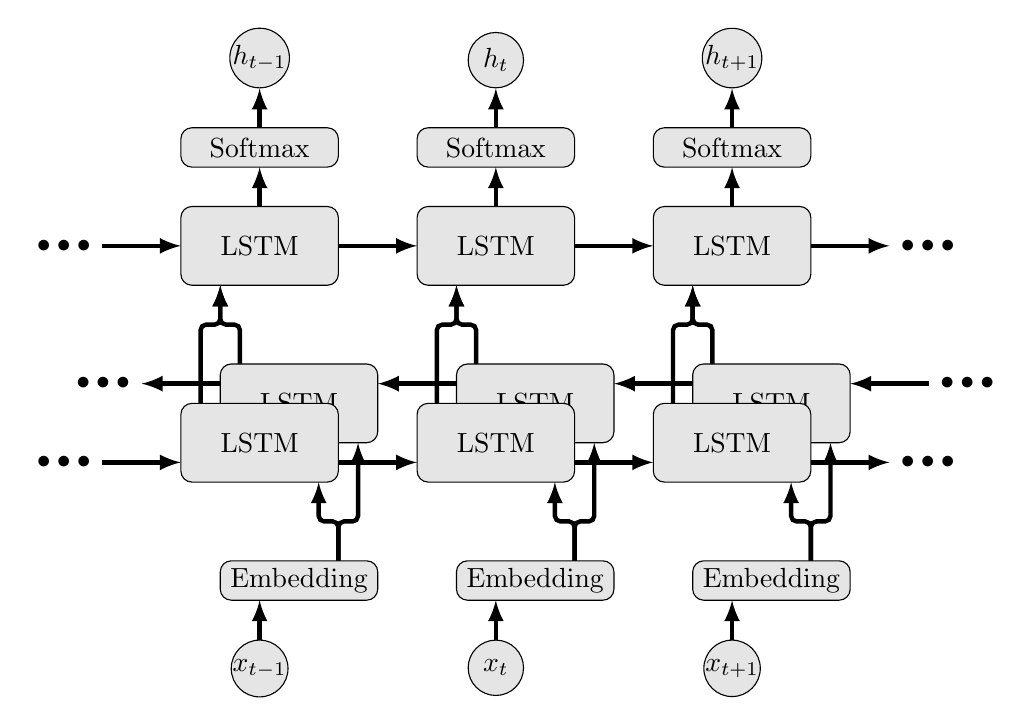
\begin{tikzpicture}[inputoutput/.style={circle, draw=black, fill=black!10, inner sep=0pt, minimum size=20pt, thin}]

% Output 
	\draw[-latex, ultra thick] (-2, 4.5) -- (-2, 5) node[inputoutput, anchor=south] {$h_{t-1}$};
	\draw[-latex, ultra thick] (1, 4.5) -- (1, 5) node[inputoutput, anchor=south] {$h_{t}$};
	\draw[-latex, ultra thick] (4, 4.5) -- (4, 5) node[inputoutput, anchor=south] {$h_{t+1}$};

% Softmax	
	\draw[rounded corners, fill=black!10] (-3, 4) rectangle (-1, 4.5) node[pos=.5] {Softmax};
	\draw[rounded corners, fill=black!10] (0, 4) rectangle (2, 4.5) node[pos=.5] {Softmax};
	\draw[rounded corners, fill=black!10] (3, 4) rectangle (5, 4.5) node[pos=.5] {Softmax};
	
	\draw[-latex, ultra thick] (-2, 3.5) -- (-2, 4);
	\draw[-latex, ultra thick] (1, 3.5) -- (1, 4);
	\draw[-latex, ultra thick] (4, 3.5) -- (4, 4);
	
% Forward lstm
	\draw[rounded corners, fill=black!10] (-3, 2.5) rectangle (-1, 3.5) node[pos=.5] {LSTM};
	\draw[rounded corners, fill=black!10] (0, 2.5) rectangle (2, 3.5) node[pos=.5] {LSTM};
	\draw[rounded corners, fill=black!10] (3, 2.5) rectangle (5, 3.5) node[pos=.5] {LSTM};
	
	\draw[-latex, ultra thick] (-4, 3) -- (-3, 3) node[pos=0, left]{$\bullet\bullet\bullet$};
	\draw[-latex, ultra thick] (-1, 3) -- (0, 3);
	\draw[-latex, ultra thick] (2, 3) -- (3, 3);
	\draw[-latex, ultra thick] (5, 3) -- (6, 3) node[right]{$\bullet\bullet\bullet$};

	\draw[-latex, ultra thick, rounded corners=2pt] (-2.75, 1) |- (-2.5, 2) -- (-2.5, 2.5);
	\draw[-latex, ultra thick, rounded corners=2pt] (-2.25, 1.5) |- (-2.5, 2) -- (-2.5, 2.5);
	
	\draw[-latex, ultra thick, rounded corners=2pt] (0.25, 1) |- (0.5, 2) -- (0.5, 2.5);
	\draw[-latex, ultra thick, rounded corners=2pt] (0.75, 1.5) |- (0.5, 2) -- (0.5, 2.5);
	
	\draw[-latex, ultra thick, rounded corners=2pt] (3.25, 1) |- (3.5, 2) -- (3.5, 2.5);
	\draw[-latex, ultra thick, rounded corners=2pt] (3.75, 1.5) |- (3.5, 2) -- (3.5, 2.5);

% Bidirectional lstm	
	\draw[rounded corners, fill=black!10] (-2.5, 0.5) rectangle (-0.5, 1.5) node[pos=.5] {LSTM};
	\draw[rounded corners, fill=black!10] (0.5, 0.5) rectangle (2.5, 1.5) node[pos=.5] {LSTM};
	\draw[rounded corners, fill=black!10] (3.5, 0.5) rectangle (5.5, 1.5) node[pos=.5] {LSTM};
	
	\draw[latex-, ultra thick] (-3.5, 1.25) -- (-2.5, 1.25) node[pos=0, left]{$\bullet\bullet\bullet$};
	\draw[latex-, ultra thick] (-0.5, 1.25) -- (0.5, 1.25);
	\draw[latex-, ultra thick] (2.5, 1.25) -- (3.5, 1.25);
	\draw[latex-, ultra thick] (5.5, 1.25) -- (6.5, 1.25) node[right]{$\bullet\bullet\bullet$};
	
	\draw[rounded corners, fill=black!10] (-3, 0) rectangle (-1, 1) node[pos=.5] {LSTM};
	\draw[rounded corners, fill=black!10] (0, 0) rectangle (2, 1) node[pos=.5] {LSTM};
	\draw[rounded corners, fill=black!10] (3, 0) rectangle (5, 1) node[pos=.5] {LSTM};
	
	\draw[-latex, ultra thick] (-4, 0.25) -- (-3, 0.25) node[pos=0, left]{$\bullet\bullet\bullet$};
	\draw[-latex, ultra thick] (-1, 0.25) -- (0, 0.25);
	\draw[-latex, ultra thick] (2, 0.25) -- (3, 0.25);
	\draw[-latex, ultra thick] (5, 0.25) -- (6, 0.25) node[right]{$\bullet\bullet\bullet$};

	\draw[-latex, ultra thick, rounded corners=2pt] (-1,-1) -- (-1, -0.5) -| (-1.25, 0);
	\draw[-latex, ultra thick, rounded corners=2pt] (-1,-1) -- (-1, -0.5) -| (-0.75, 0.5);
	
	\draw[-latex, ultra thick, rounded corners=2pt] (2,-1) -- (2, -0.5) -| (1.75, 0);
	\draw[-latex, ultra thick, rounded corners=2pt] (2,-1) -- (2, -0.5) -| (2.25, 0.5);
	
	\draw[-latex, ultra thick, rounded corners=2pt] (5,-1) -- (5, -0.5) -| (4.75, 0);
	\draw[-latex, ultra thick, rounded corners=2pt] (5,-1) -- (5, -0.5) -| (5.25, 0.5);

% embedding layer

	\draw[rounded corners, fill=black!10] (-2.5, -1.5) rectangle (-0.5, -1) node[pos=.5] {Embedding};
	\draw[rounded corners, fill=black!10] (0.5, -1.5) rectangle (2.5, -1) node[pos=.5] {Embedding};
	\draw[rounded corners, fill=black!10] (3.5, -1.5) rectangle (5.5, -1) node[pos=.5] {Embedding};

% Input layer	
	\draw[-latex, ultra thick] (-2, -2) -- (-2, -1.5) node[inputoutput, pos=0, anchor=north] {$x_{t-1}$};
	\draw[-latex, ultra thick] (1, -2) -- (1, -1.5) node[inputoutput, pos=0, anchor=north] {$x_{t}$};
	\draw[-latex, ultra thick] (4, -2) -- (4, -1.5) node[inputoutput, pos=0, anchor=north] {$x_{t+1}$};			
	\end{tikzpicture}
	\caption{The layers for the model of step 1}
	\label{fig:step1}
\end{figure}

The model for step 1 consists of an embedding layer with a bidirectional \gls{lstm} on top followed by a
forward \gls{lstm} and a softmax layer on top to give a probability distribution of the output classes.
An illustration of the model for step 1 can be seen in Figure \ref{fig:step1}.

The embedding layer is a matrix that transform the input from discrete integers to dense vectors, 
this serves two purposes. The first and most important purpose is to embed the discrete input values 
into a continues vector space. The input is integers from 0 to 19 corresponding to the amino acids, but 
these are discrete and have no concept of distance. By embedding them into a continues vector space 
it becomes possible to compute a distance between points,
and the matrix can be altered by the training of the network, 
the idea is the network learns to embed similar amino acids to similar regions in the vector space
and with multiple dimension, different dimension could represent different measures for similarity. 
The measures for similarity is not necessarily something that makes sense to a human but just whatever 
gives the best results. The second purpose is to project the dimensionality of the input to something else 
to be able to chose the size of the next layer. This could be done by a projection layer but with an embedding 
layer this is unnecessary. 

After the embedding layer comes a bidirectional \gls{lstm}. This consists of two parallel \glspl{lstm} where 
one is an ordinary forward \gls{lstm} and the other is a backward \gls{lstm} that starts at the end of the 
input sequence and goes though it to the start. The output from the two \glspl{lstm} is then concatenated
such that the total output is a sequence of element wise concatenated output corresponding to the same input.
The reason for this layer to be bidirectional is that each element in the output now consists of information
gathered from both before and after the element's position. 

On top of the bidirectional \gls{lstm} is an ordinary forward \gls{lstm} to do some computation on the
gathered information. This layer does not benefit from being bidirectional because it already have 
information from both directions. It does however benefit from being a recurrent layer, not 
because it can remember earlier input, but because it can remember earlier output and therefore have
information about the number of consecutive output of the same class. This layer does not actually 
output the classes, but a vector used to compute the probability distribution.

The last layer is softmax layer. This is an ordinary non-recurrent fully-connected layer, same as in 
a \gls{mlp}. This layer uses the softmax function as activation function to be able to output 
a probability distribution of the output classes.
 
\subsubsection{Step 2}

\begin{figure}
	\centering
	\begin{BVerbatim}
Sequence:       ...CDVVVVGGGISGMA...
True structure: ...nnnnnnnnnnnnnn...
Before step 2:  ...nnHHHHnnnnHHnn...
After step 2:   ...nnnnnnnnnnnnnn...
	\end{BVerbatim}
	\caption{A prediction containing noise}
	\label{fig:noisy_prediction}
\end{figure}

Step 2 is not a machine learning model, but a post processing of the output of step 1. The output from 
step 1 contains a lot of noise in the form of sudden short peaks for some classes and regions where the 
model is uncertain of which class the positions belong to which causes the predicted structure to contain
regions with changing classes as can be seen in Figure \ref{fig:noisy_prediction}. The purpose of step 2
is to remove as much as possible of this noise without removing good parts of the prediction.
This is done, as in TMSEG, by first averaging each position from a window of size five around the position.
After this is consecutive sequences of \glspl{tmh} shorter than seven, changed into non-\gls{tmh}. 

I did not apply penalties to each class as they did in TMSEG, because the values was empirical determined 
and specific to their model. It would maybe be possible to remove some of the uncertainty by applying
penalties, but could as well function as a bias for how sure the model should be in a prediction instead 
of giving the best average result, I have therefore chosen to not use time on this.

\subsubsection{Step 3}
The layout of the model for step 3 is almost identical to the model for step 1, the only difference
in the layout is the input to the softmax layer is the cell-state of the previous \gls{lstm} layer
instead of the sequence output. This is done because the model's purpose is to make prediction on
the whole input and not on each position. The biggest difference to step 1 is not in the layout,
but in the purpose and therefore the input and training. The purpose of step 3 is to adjust the 
endpoints of a \gls{tmh} and this is done, like in TMSEG, by taking a segment of the sequence 
and training the model to determine the probability of that segment to be a \gls{tmh}. 
This is used to adjust the endpoints by generating segments by shifting the endpoints of the 
previous predicted \gls{tmh} and using the model to determine which segment has the highest
probability of being a \gls{tmh}. The training og this model is done by making these segments for
the \glspl{tmh} in the true structure and labelling the the segments of the true \glspl{tmh} as \gls{tmh}
and the others as non-\gls{tmh}. 

\subsection{Machine Learning Libraries}
A lot of different machine learning libraries exists, like Tensorflow\cite{tensorflow}, Caffe\cite{caffe}, 
Theano\cite{theano} and more. These can make the implementations of a machine learning model a lot easier 
and faster. I have chosen to use Tensorflow mostly because I had prior knowledge and experience with it.

With tensorflow you first define a computation graph for the model and then you run the graph.
This has the advantages that the graph is just a data structure and therefore can be language and platform 
independent, and the defining of the computation graph and the running of it can be separated to different 
processes. The running can therefore be handled by a highly optimized back-end and the defining can be done 
by using an API in a different language.
The library also adds a lot of modules that can be used together as blocks to form large parts of the 
computation graph. Most standard components of machine learning models, like different layer types, 
loss functions, training algorithms and even multiple different implementations of \gls{lstm} cells.
This gives the ability to concentrate on non standard parts of the model that is associated to the 
problem instance and not the type of machine learning used, like pre- and post-processing of in- and output.

\subsection{Implementation}
The Tensorflow api for Python is the most stable and complete, I have therefore chosen to use 
the language Python to implement the model in. As mentioned earlier, Tensorflow comes with 
implementations of most machine learning components, for example a \gls{lstm} layer can 
be added to the combutation graph by first specifying the hyper-parameters, like the size
which is called \texttt{num\_units}, which is done by the following lines of code:

\begin{lstlisting}[language=Python]
fw_lstm = tf.contrib.rnn.LSTMBlockFusedCell(
    num_units=num_units,
    forget_bias=0,
    cell_clip=None,
    use_peephole=False)
\end{lstlisting}

thereafter the initial state has to be specified, which could be zeros or the state from the last 
input. If each input have some connection it could make sense to use the state from last, 
of course it has to start with something at some point. I have chosen to start fresh with zeroes 
with each new sequence. As mentioned in section \ref{sec:lstm}, the state consists of two parts
the cell-state, $C$, and the previous output, $h$, the code to create the initial state therefore 
becomes:

\begin{lstlisting}[language=Python]
initial_state = (
    tf.zeros([batch_size, num_units], tf.float32),
    tf.zeros([batch_size, num_units], tf.float32))
\end{lstlisting}

Then to add the layer to the graph, the input node called \texttt{input\_tensor}, the initial state, 
and a node containing the lengths of the input sequences has to be specified, which is done by:

\begin{lstlisting}[language=Python]
output, state = fw_lstm(input_tensor,
                        initial_state=initial_state,
                        dtype=None,
                        sequence_length=lengths,
                        scope="lstm")
\end{lstlisting}

This gives a graph node, \texttt{output}, containing the output from the  layer, which can be used
as input on the next layer. Different layers can be added in a similar way. It is therefore not 
the most complicated part of the model that is the most difficult to implement, but the parts
that is specific to this model, like pre- and post-processing of the data. Tensorflow is designed 
to make it easy to do linear algebra on tensors, which is a collection of matrices. This is the 
reason it is easy to implement \glspl{ann} in Tensorflow, but tasks like the filters applied by 
step 2 and the generation of segments in step 3 cannot be expressed as linear algebra and is 
therefore not as easy to implement with tensorflow. Most of the work of implementing the model
therefore lies in these parts. 
The code can be found on:
\begin{verbatim}
	https://github.com/lynderup/Kasper_Speciale_2017
\end{verbatim}


